
\documentclass[12pt, a4paper]{article}
\usepackage{../../../myconfig} % Gọi file cấu hình từ ngoài gốc vào

% ==========================================
% BẮT ĐẦU NỘI DUNG TÀI LIỆU
% ==========================================
\begin{document}

% Truyền 3 tham số: {Nhãn cam} {Chữ to chính giữa} {Chữ ở góc phải Header}
\titlebox{Chủ đề: Tích phân}{Ứng dung tích phân tính diện hình phẳng thực tế}{Nguyên hàm - Tích phân: Ứng dụng}

\drawdashlines{27}
\newpage
\drawdashlines{35}

\questionLinesManual{23}{1}{Ông An muốn làm cửa rào sắt có hình dạng và kích thước như hình vẽ bên, biết đường cong phía trên là một Parabol.  
Giá \( 1(m^2) \) của rào sắt là 700.000 đồng.  
Hỏi ông An phải trả bao nhiêu tiền để làm cái cửa sắt như vậy (làm tròn đến hàng phần nghìn).
\begin{figure}[htbp]
    \centering
    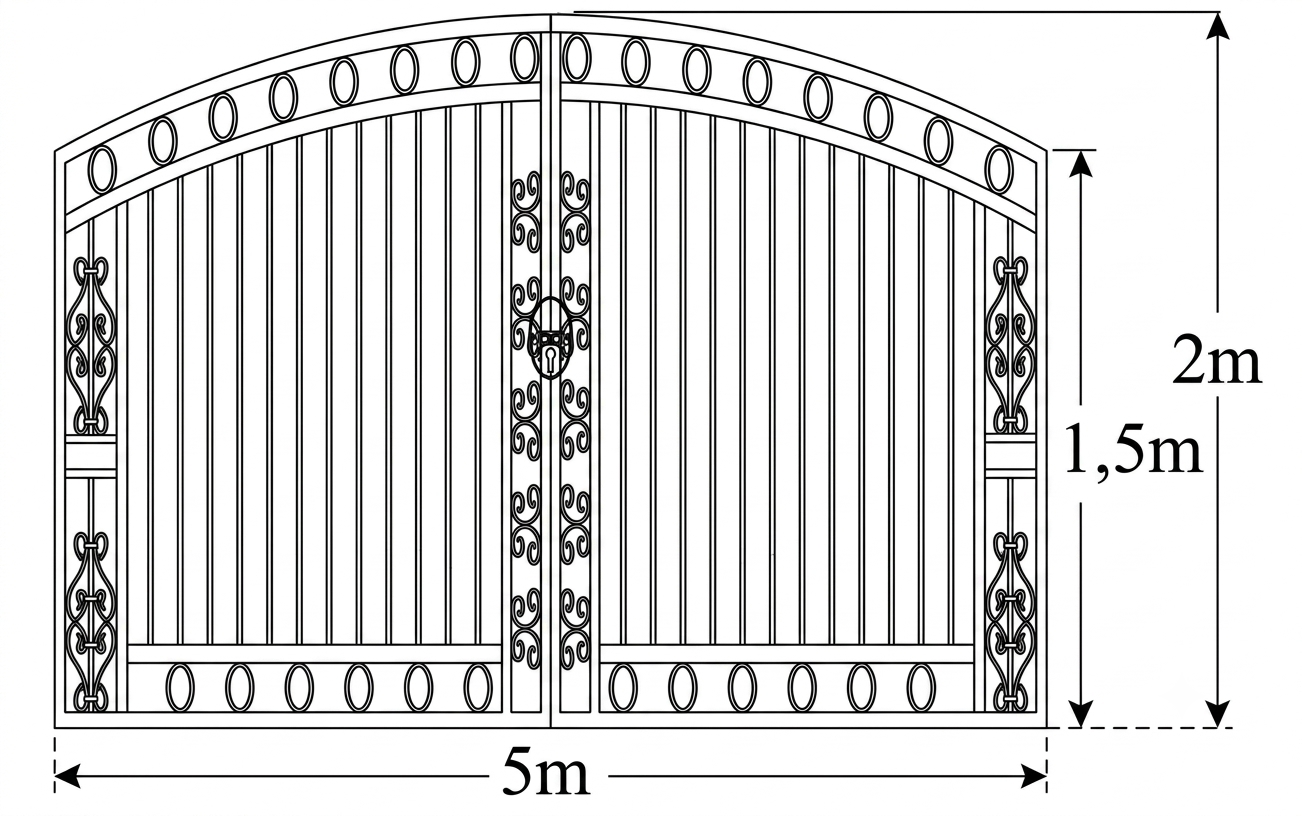
\includegraphics[width=0.4\textwidth]{../images/Cong.png}
\end{figure}

}{%
    \begin{tasks}(4)
        \task 6.520.000 đồng
        \task 6.320.000 đồng
        \task 6.417.000 đồng
        \task 6.620.000 đồng
    \end{tasks}
}

\questionShortAnswer{23}{2}{Trang trí một sân hình chữ nhật kích thước 30m × 16m, trong đó hai Parabol \( (P_1) \) đối xứng với \( (P_2) \) qua đường thẳng đi qua hai trung điểm của chiều dài sân (hình vẽ), khoảng cách giữa hai đỉnh Parabol bằng 6m.  
Chi phí trang trí cho phần hoa văn là 200 ngàn đồng trên một mét vuông, phần trắng là 180 ngàn đồng trên một mét vuông. Tổng chi phí trang trí cho sân là bao nhiêu triệu đồng (kết quả làm tròn đến hàng phần mười)?

\begin{center}
\begin{tikzpicture}[scale=0.25, >=latex]
    % Khai báo thư viện \usetikzlibrary{patterns} ở Preamble

    % 1. Tô họa tiết ô caro cho phần hoa văn
    \begin{scope}
        % Tô toàn bộ hình chữ nhật bằng mẫu caro (checkerboard)
        \fill[pattern=checkerboard, pattern color=black!60] (-15,-8) rectangle (15,8);

        \fill[white] (15,-8) -- plot[domain=-8:-3, samples=100] ({0.28*\x*\x - 3}, \x) -- plot[domain=-3:3, samples=100] ({-0.28*\x*\x + 3}, \x) -- plot[domain=3:8, samples=100] ({0.28*\x*\x - 3}, \x) -- (15,8) -- cycle;

        \fill[white] (-15,-8) -- plot[domain=-8:-3, samples=100] ({-0.28*\x*\x + 3}, \x) -- plot[domain=-3:3, samples=100] ({0.28*\x*\x - 3}, \x) -- plot[domain=3:8, samples=100] ({-0.28*\x*\x + 3}, \x) -- (-15,8) -- cycle;
            \end{scope}

    % 2. Vẽ viền khung hình chữ nhật 30x16
    \draw[very thick] (-15,-8) rectangle (15,8);

    % 3. Vẽ hai đường Parabol (P1) và (P2)
    \draw[very thick, samples=100, domain=-8:8] plot ({-0.28*\x*\x +3}, \x);
    \draw[very thick, samples=100, domain=-8:8] plot ({0.28*\x*\x - 3}, \x);

    % 4. Đánh dấu nhãn (P1) và (P2)
    \node at (-7, 3) {\small $(P_1)$};
    \node at (7, 3) {\small $(P_2)$};
\end{tikzpicture}
\end{center}
}

\questionLinesManual{22}{3}{Một mảnh vườn hình tròn tâm \( O \) bán kính \( 6 \, \text{m} \). Người ta cần trồng cây trên dải đất rộng \( 6 \, \text{m} \) nhận \( O \) làm tâm đối xứng, biết kinh phí trồng cây là \( 70000 \, \text{đồng/m}^2 \). Hỏi cần bao nhiêu tiền để trồng cây trên dải đất đó (số tiền được làm tròn đến hàng đơn vị)
\begin{center}
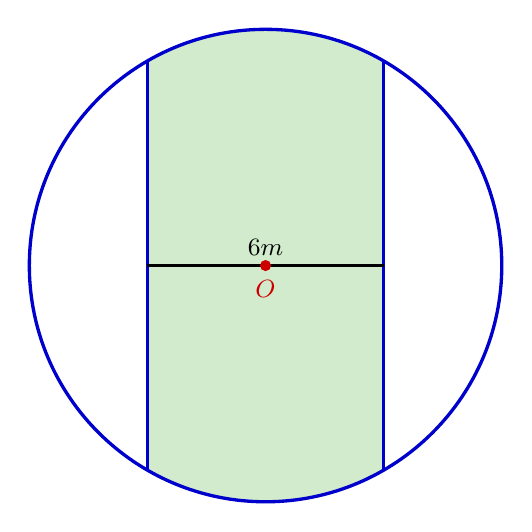
\begin{tikzpicture}[scale=0.5, >=latex]
    % Định nghĩa màu xanh lá nhạt cho dải đất
    \definecolor{gardenlight}{RGB}{210, 235, 205}

    % 1. Tô màu dải đất rộng 6m trong hình tròn R = 6
    \begin{scope}
        \clip (0,0) circle (6);
        \fill[gardenlight] (-3,-6) rectangle (3,6);
    \end{scope}

    % 2. Viền đường tròn bán kính 6m
    \draw[very thick, blue!80!black] (0,0) circle (6);

    % 3. Khung biên hai bên của dải đất
    \begin{scope}
        \clip (0,0) circle (6);
        \draw[very thick, blue!80!black] (-3,-6) -- (-3,6);
        \draw[very thick, blue!80!black] (3,-6) -- (3,6);
    \end{scope}

    % 4. Đoạn thẳng biểu diễn độ rộng 6m qua tâm O
    \draw[thick] (-3,0) -- (3,0) node[midway, above] {\small $6\text{m}$};
    \fill[red!80!black] (0,0) circle (4pt) node[below=2pt] {\small $O$};
\end{tikzpicture}
\end{center}
}{%
    \begin{tasks}(4)
        \task 8.412.322 đồng
        \task 8.142.232 đồng
        \task 4.821.232 đồng
        \task 4.821.322 đồng
    \end{tasks}
}

\questionLinesManual{22}{4}{Một khuôn viên dạng nửa hình tròn, trên đó người thiết kế phần để trồng hoa có dạng của một cánh hoa hình parabol có đỉnh trùng với tâm và có trục đối xứng vuông góc với đường kính của nửa hình tròn, hai đầu mút của cánh hoa nằm trên nửa đường tròn (phần tô màu) và cách nhau một khoảng bằng \( 4(m) \). Phần còn lại của khuôn viên (phần không tô màu) dành để trồng cỏ Nhật Bản. Biết các kích thước cho như hình vẽ, chi phí để trồng hoa và cỏ Nhật Bản tương ứng là 150.000 đồng/m² và 100.000 đồng/m². Hỏi cần bao nhiêu tiền để trồng hoa và trồng cỏ Nhật Bản trong khuôn viên đó? (Số tiền được làm tròn đến hàng đơn vị)
\begin{center}
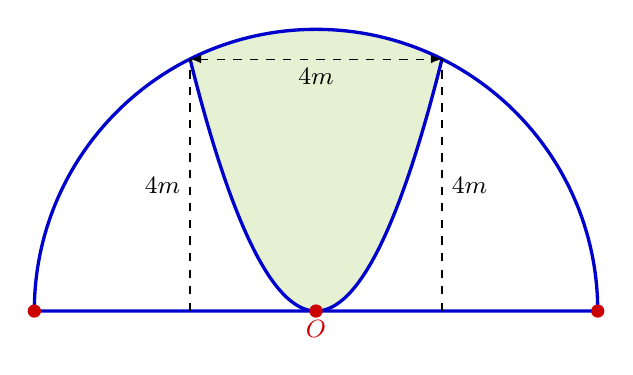
\begin{tikzpicture}[scale=0.8, >=latex]
    % Định nghĩa bán kính R = sqrt(20) ~ 4.47
    \pgfmathsetmacro{\R}{sqrt(20)}

    % 1. Tô màu xám/vàng cam nhạt cho phần trồng hoa (Parabol đến nửa đường tròn)
    \definecolor{flowercolor}{RGB}{230, 240, 210}
    \fill[flowercolor] 
        plot[domain=-2:2, samples=100] (\x, {\x*\x}) -- 
        plot[domain=2:-2, samples=100] (\x, {sqrt(20 - \x*\x)}) -- cycle;

    % 2. Viền nửa đường tròn
    \draw[very thick, blue!80!black] (-\R, 0) arc (180:0:\R) -- cycle;

    % 3. Vẽ Parabol y = x^2
    \draw[very thick, blue!80!black, domain=-2:2, samples=100] plot (\x, {\x*\x});

    % 4. Các đường dóng kích thước đứt nét
    \draw[dashed] (-2,0) -- (-2,4);
    \draw[dashed] (2,0) -- (2,4);
    \draw[dashed, <->] (-2,4) -- (2,4) node[midway, below] {\small $4\text{m}$};

    % 5. Nhãn kích thước chiều cao 4m
    \node[left] at (-2,2) {\small $4\text{m}$};
    \node[right] at (2,2) {\small $4\text{m}$};

    % 6. Các điểm mút và gốc O
    \fill[red!80!black] (0,0) circle (3pt) node[below] {\small $O$};
    \fill[red!80!black] (-\R,0) circle (3pt);
    \fill[red!80!black] (\R,0) circle (3pt);
\end{tikzpicture}
\end{center}
}{%
    \begin{tasks}(4)
        \task 3.738.574 đồng
        \task 1.948.000 đồng
        \task 3.926.990 đồng
        \task 4.115.408 đồng
    \end{tasks}
}

\questionLinesManual{22}{5}{Một biển quảng cáo có dạng hình elip với bốn đỉnh \( A_1, A_2, B_1, B_2 \) như hình vẽ bên. Biết chi phí để sơn phần tô đậm là 200.000 vnđ/m² và phần còn lại 100.000 vnđ/m². Hỏi số tiền để sơn theo cách trên gần nhất với số tiền nào dưới đây, biết \( A_1A_2 = 8m \), \( B_1B_2 = 6m \) và tứ giác \( MNPQ \) là hình chữ nhật có \( MQ = 3m \)?

\begin{center}
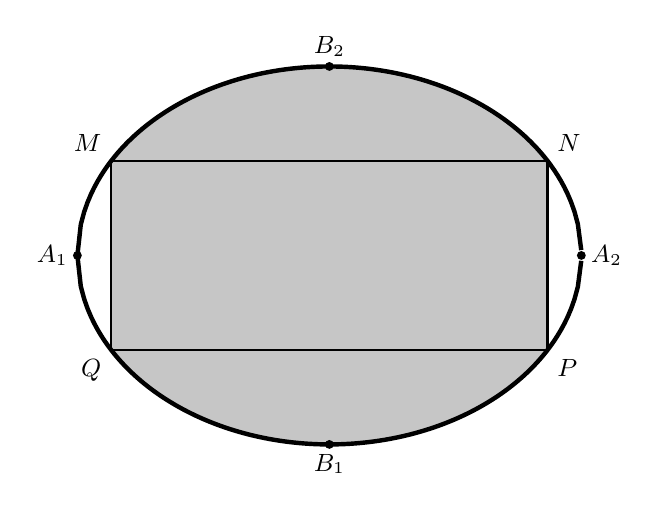
\begin{tikzpicture}[scale=0.8, >=latex]
    % Định nghĩa bán trục
    \pgfmathsetmacro{\a}{4}
    \pgfmathsetmacro{\b}{3}
    \pgfmathsetmacro{\xM}{sqrt(12)} % 2*sqrt(3) ~ 3.464
    \pgfmathsetmacro{\yM}{1.5}

    % 1. Tô phần tô đậm (phần giữa hình chữ nhật và elip)
    \fill[color=gray!45, domain=-\xM:\xM, variable=\x]
        plot (\x, {3*sqrt(1 - \x*\x/16)}) -- 
        plot (\x, {1.5}) -- cycle;
    \fill[color=gray!45, domain=-\xM:\xM, variable=\x]
        plot (\x, {-1.5}) -- 
        plot (\x, {-3*sqrt(1 - \x*\x/16)}) -- cycle;

    % 2. Tô màu xám đậm cho phần hình chữ nhật MNPQ
    \fill[gray!45] (-\xM, -\yM) rectangle (\xM, \yM);

    % 3. Vẽ đường Elip
    \draw[ultra thick, samples=150, domain=-4:4, color=black] 
        plot (\x, {3*sqrt(1 - \x*\x/16)});
    \draw[ultra thick, samples=150, domain=-4:4, color=black] 
        plot (\x, {-3*sqrt(1 - \x*\x/16)});

    % 4. Viền hình chữ nhật MNPQ
    \draw[thick] (-\xM, -\yM) rectangle (\xM, \yM);

    % 5. Đánh dấu các đỉnh của Elip
    \fill[black] (-\a,0) circle (2pt) node[left] {\small $A_1$};
    \fill[black] (\a,0) circle (2pt) node[right] {\small $A_2$};
    \fill[black] (0,-\b) circle (2pt) node[below] {\small $B_1$};
    \fill[black] (0,\b) circle (2pt) node[above] {\small $B_2$};

    % 6. Đánh dấu các đỉnh hình chữ nhật
    \node[above left] at (-\xM, \yM) {\small $M$};
    \node[above right] at (\xM, \yM) {\small $N$};
    \node[below right] at (\xM, -\yM) {\small $P$};
    \node[below left] at (-\xM, -\yM) {\small $Q$};
\end{tikzpicture}
\end{center}
}{%
    \begin{tasks}(4)
        \task 5.526.000 đồng
        \task 5.782.000 đồng
        \task 7.322.000 đồng
        \task 7.213.000 đồng
    \end{tasks}
}

\questionLinesManual{22}{6}{Một sân chơi cho trẻ em hình chữ nhật có chiều dài 100 và chiều rộng là 60 m người ta làm một con đường nằm trong sân (như hình vẽ). Biết rằng viền ngoài và viền trong của con đường là hai đường elip, Elip của đường viền ngoài có trục lớn và trục bé lần lượt song song với các cạnh hình chữ nhật và chiều rộng của mặt đường là 2 m. Kinh phí cho mỗi m\(^2\) làm đường 600.000 đồng. Tính tổng số tiền làm con đường đó. (Số tiền được làm tròn đến hàng nghìn).

\begin{center}
\begin{tikzpicture}[scale=0.08, >=latex]
    % Định nghĩa tham số bán trục
    \pgfmathsetmacro{\aOuter}{50}
    \pgfmathsetmacro{\bOuter}{30}
    \pgfmathsetmacro{\aInner}{42}
    \pgfmathsetmacro{\bInner}{22}

    % Khai báo họa tiết và màu sắc
    \definecolor{grassgreen}{RGB}{120, 180, 100}
    \definecolor{innercream}{RGB}{254, 245, 215}

    % 1. Tô màu nền xanh cho sân chơi
    \fill[grassgreen] (-\aOuter, -\bOuter) rectangle (\aOuter, \bOuter);

    % 2. Tô họa tiết kim cương/caro cho dải đường elip giữa 2 elip
    \begin{scope}
        % Cắt vùng nằm trong Elip ngoài
        \clip plot[domain=0:360, samples=120] ({\aOuter*cos(\x)}, {\bOuter*sin(\x)});
        
        % Tô màu nền họa tiết
        \fill[pattern=checkerboard, pattern color=green!70!black!40] (-\aOuter, -\bOuter) rectangle (\aOuter, \bOuter);
        
        % Xóa màu lòng trong bằng Elip nhỏ
        \fill[innercream] plot[domain=0:360, samples=120] ({\aInner*cos(\x)}, {\bInner*sin(\x)});
    \end{scope}

    % 3. Vẽ 2 đường Elip bằng hàm Parametric (plot)
    % Elip ngoài
    \draw[ultra thick, domain=0:360, samples=120] 
        plot ({\aOuter*cos(\x)}, {\bOuter*sin(\x)});

    % Elip trong
    \draw[ultra thick, domain=0:360, samples=120] 
        plot ({\aInner*cos(\x)}, {\bInner*sin(\x)});

    % 4. Khung hình chữ nhật bao ngoài
    \draw[ultra thick] (-\aOuter, -\bOuter) rectangle (\aOuter, \bOuter);

    % 5. Mũi tên đo kích thước
    \draw[<->, thick] (-\aOuter, \bOuter + 5) -- (\aOuter, \bOuter + 5) 
        node[midway, fill=white, inner sep=2pt] {\large $100\text{m}$};
        
    \draw[<->, thick] (-\aOuter - 5, -\bOuter) -- (-\aOuter - 5, \bOuter) 
        node[midway, fill=white, inner sep=1pt] { $60\text{m}$};
        
    \draw[<->, thick] (0, \bInner) -- (0, \bOuter) 
        node[midway, right] {\large $2\text{m}$};
\end{tikzpicture}
\end{center}
}{%
    \begin{tasks}(4)
        \task 293.904.000 đồng
        \task 283.904.000 đồng
        \task 293.804.000 đồng
        \task 283.604.000 đồng
    \end{tasks}
}


\end{document}